%%%%%%%%%%%%%%%%%%%%%%%%
%
% $Autor: Hemanth Jadiswami Prabhakaran $
% $Datum: 2025-06-30 11:19:18Z $
% $Pfad: GitHub/BA25-01-Time-Series/Manual/Chapters/en/06SystemSpecifications.tex $
% $Version: 1 $
%
% $Project: BA25-Time-Series $
%
%%%%%%%%%%%%%%%%%%%%%%%%



\chapter{System Specifications}

\section{Technical Requirements Overview}

The Walmart Sales Forecasting System is designed to operate across multiple deployment environments while maintaining consistent performance and functionality. This chapter provides comprehensive technical specifications for both local installation and cloud deployment scenarios.

\begin{figure}[H]
	\centering
	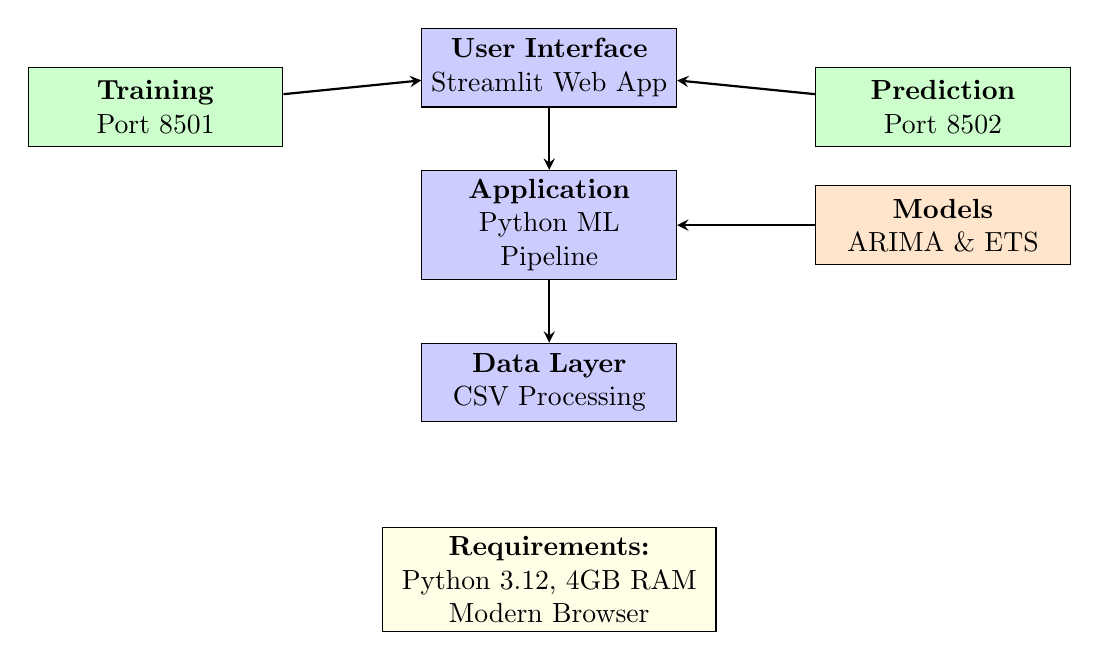
\begin{tikzpicture}[
	box/.style={rectangle, draw, fill=blue!20, text width=3cm, text centered, minimum height=1cm},
	arrow/.style={thick,->,>=stealth}
	]
	
	% Title

	
	% Main layers
	\node[box] (ui) at (0,3) {\textbf{User Interface}\\Streamlit Web App};
	
	\node[box] (app) at (0,1) {\textbf{Application}\\Python ML Pipeline};
	
	\node[box] (data) at (0,-1) {\textbf{Data Layer}\\CSV Processing};
	
	% Side components
	\node[box, fill=green!20] (train) at (-5,2.5) {\textbf{Training}\\Port 8501};
	
	\node[box, fill=green!20] (predict) at (5,2.5) {\textbf{Prediction}\\Port 8502};
	
	\node[box, fill=orange!20] (models) at (5,1) {\textbf{Models}\\ARIMA \& ETS};
	
	% Arrows
	\draw[arrow] (ui) -- (app);
	\draw[arrow] (app) -- (data);
	\draw[arrow] (train) -- (ui);
	\draw[arrow] (predict) -- (ui);
	\draw[arrow] (models) -- (app);
	
	% Requirements box
	\node[box, fill=yellow!10, text width=4cm] at (0,-3.5) {
		\textbf{Requirements:}\\
		Python 3.12, 4GB RAM\\
		Modern Browser
	};
	
\end{tikzpicture}
	\caption{System Technical Architecture and Requirements}
	\label{fig:technical_architecture}
\end{figure}

\section{Local Installation Requirements}

\subsection{Core System Requirements}

\textbf{Python Environment}
\begin{itemize}
	\item \textbf{Python Version}: Exactly Python 3.12.x (3.12.0, 3.12.1, 3.12.2, etc.)
	\item \textbf{Version Restriction}: NOT compatible with Python 3.13+ or Python 3.11 and below
	\item \textbf{Architecture}: 64-bit Python installation required
	\item \textbf{Installation Source}: Official Python.org distribution recommended
\end{itemize}

\textbf{Operating System Support}
\begin{itemize}
	\item \textbf{Windows}: Windows 10 (version 1903+) or Windows 11
	\item \textbf{macOS}: macOS 10.15 (Catalina) or newer
	\item \textbf{Linux}: Ubuntu 18.04+, CentOS 7+, or equivalent distributions
	\item \textbf{Architecture}: x86\_64 (AMD64) processor architecture
\end{itemize}

\begin{table}[H]
	\centering
	\begin{tabularx}{\textwidth}{|X|X|X|}
		\hline
		\textbf{Component} & \textbf{Minimum} & \textbf{Recommended} \\
		\hline
		CPU & Dual-core 2.0 GHz & Quad-core 3.0 GHz+ \\
		RAM & 4 GB & 8 GB or more \\
		Storage & 2 GB free space & 5 GB free space \\
		Network & 1 Mbps & 10 Mbps+ \\
		\hline
	\end{tabularx}
	\caption{Hardware Requirements for Local Installation}
	\label{tab:hardware_requirements}
\end{table}

\subsection{Software Dependencies}

\textbf{Required Python Packages}

The system depends on specific package versions for stability and compatibility:

\begin{table}[H]
	\centering
	\begin{tabularx}{\textwidth}{|X|X|X|}
		\hline
		\textbf{Package} & \textbf{Version} & \textbf{Purpose} \\
		\hline
		streamlit & 1.32.0 & Web application framework \\
		pandas & 2.2.2 & Data manipulation and analysis \\
		numpy & 1.26.4 & Numerical computing foundation \\
		matplotlib & 3.8.4 & Static plotting and visualization \\
		seaborn & 0.13.2 & Statistical data visualization \\
		plotly & 5.24.1 & Interactive web-based plotting \\
		joblib & 1.4.2 & Model serialization and loading \\
		statsmodels & 0.14.2 & Statistical modeling library \\
		pmdarima & 2.0.4 & Auto ARIMA implementation \\
		pytest & 7.4.4 & Testing framework for validation \\
		\hline
	\end{tabularx}
	\caption{Required Python Package Dependencies}
	\label{tab:python_dependencies}
\end{table}

\textbf{Virtual Environment Configuration}

\begin{lstlisting}[language=bash]
	# Virtual environment creation
	python3.12 -m venv walmart_forecast_env
	
	# Environment activation (Linux/macOS)
	source walmart_forecast_env/bin/activate
	
	# Environment activation (Windows)
	walmart_forecast_env\Scripts\activate
	
	# Package installation
	pip install -r requirements.txt
\end{lstlisting}

\subsection{Port and Network Configuration}

\textbf{Default Port Assignments}
\begin{itemize}
	\item \textbf{Training Application}: Port 8501 (Streamlit default)
	\item \textbf{Prediction Application}: Port 8502 (manually configured)
	\item \textbf{Protocol}: HTTP (local development only)
	\item \textbf{Firewall}: No special firewall configuration required for local use
\end{itemize}

\textbf{Network Requirements}
\begin{itemize}
	\item \textbf{Internet Access}: Required for initial package installation
	\item \textbf{Bandwidth}: Minimal during operation (interface assets only)
	\item \textbf{Latency}: Not critical for local deployment
	\item \textbf{Proxy}: Compatible with corporate proxy configurations
\end{itemize}

\section{Cloud Deployment Specifications}

\subsection{Streamlit Cloud Infrastructure}

\textbf{Platform Specifications}
\begin{itemize}
	\item \textbf{Hosting Provider}: Streamlit Community Cloud
	\item \textbf{Runtime Environment}: Containerized Python 3.12 environment
	\item \textbf{Resource Allocation}: Shared compute resources with automatic scaling
	\item \textbf{Geographic Distribution}: Global CDN for optimized access speeds
\end{itemize}

\textbf{Performance Characteristics}
\begin{itemize}
	\item \textbf{CPU}: Shared vCPU with fair-use allocation
	\item \textbf{Memory}: 1GB RAM per application instance
	\item \textbf{Storage}: Ephemeral file system with session-based persistence
	\item \textbf{Bandwidth}: Unlimited for normal usage patterns
\end{itemize}

\begin{table}[H]
	\centering
	\begin{tabularx}{\textwidth}{|X|X|X|}
		\hline
		\textbf{Metric} & \textbf{Training App} & \textbf{Prediction App} \\
		\hline
		Cold Start Time & 15-45 seconds & 10-30 seconds \\
		Warm Response Time & < 2 seconds & < 1 second \\
		Session Timeout & 30 minutes idle & 30 minutes idle \\
		File Upload Limit & 200 MB & 200 MB \\
		Concurrent Users & 50+ supported & 100+ supported \\
		\hline
	\end{tabularx}
	\caption{Cloud Deployment Performance Specifications}
	\label{tab:cloud_performance}
\end{table}

\subsection{Browser Compatibility}

\textbf{Supported Browsers}
\begin{itemize}
	\item \textbf{Google Chrome}: Version 90+ (Recommended)
	\item \textbf{Mozilla Firefox}: Version 88+
	\item \textbf{Microsoft Edge}: Version 90+
	\item \textbf{Safari}: Version 14+ (macOS/iOS)
\end{itemize}

\textbf{Browser Feature Requirements}
\begin{itemize}
	\item \textbf{JavaScript}: ES6+ support required
	\item \textbf{WebSockets}: For real-time application updates
	\item \textbf{Local Storage}: For session state management
	\item \textbf{File API}: For drag-and-drop file uploads
\end{itemize}

\section{Data Format Specifications}

\subsection{Input Data Requirements}

\textbf{CSV File Structure}

The system expects three specific CSV files with predefined schemas:

\subsubsection{train.csv Requirements}
\begin{itemize}
	\item \textbf{Required Columns}: Store, Date, Weekly\_Sales, IsHoliday
	\item \textbf{Store Column}: Integer values (1, 2, 3, ...)
	\item \textbf{Date Column}: YYYY-MM-DD format (e.g., 2010-02-05)
	\item \textbf{Weekly\_Sales}: Float values representing sales in dollars
	\item \textbf{IsHoliday}: Boolean values (True/False or 1/0)
\end{itemize}

\subsubsection{features.csv Requirements}
\begin{itemize}
	\item \textbf{Required Columns}: Store, Date, Temperature, Fuel\_Price, MarkDown1-5, CPI, Unemployment, IsHoliday
	\item \textbf{Store/Date}: Same format as train.csv for proper merging
	\item \textbf{Temperature}: Float values in Fahrenheit
	\item \textbf{Fuel\_Price}: Float values in dollars per gallon
	\item \textbf{MarkDown1-5}: Float values (may contain NaN for missing markdowns)
	\item \textbf{CPI/Unemployment}: Float values for economic indicators
\end{itemize}

\subsubsection{stores.csv Requirements}
\begin{itemize}
	\item \textbf{Required Columns}: Store, Type, Size
	\item \textbf{Store}: Integer values matching train.csv and features.csv
	\item \textbf{Type}: String values (A, B, or C)
	\item \textbf{Size}: Integer values representing store square footage
\end{itemize}

\begin{figure}[H]
	\centering
	\includegraphics[width=0.9\textwidth]{Images/06SystemSpecifications/DataSchemaTrainExample.png}
	\includegraphics[width=0.9\textwidth]{Images/06SystemSpecifications/DataSchemaFeatureExample.png}
		\includegraphics[width=0.9\textwidth]{Images/06SystemSpecifications/DataSchemaStoreExample.png} 
			\caption{Example Data Schema and Format Requirements}
	\label{fig:data_schema_example}
\end{figure}

\subsection{Model File Specifications}

\textbf{Model Serialization Format}
\begin{itemize}
	\item \textbf{Primary Format}: Joblib .pkl files
	\item \textbf{Compression}: Optional gzip compression supported
	\item \textbf{Python Version}: Must be serialized with Python 3.12
	\item \textbf{Cross-Platform}: Compatible across Windows, macOS, and Linux
\end{itemize}

\textbf{Model File Structure}
\begin{itemize}
	\item \textbf{File Extension}: .pkl (required)
	\item \textbf{Naming Convention}: ModelType.pkl (e.g., AutoARIMA.pkl)
	\item \textbf{Size Limits}: Typically 1-50 MB depending on model complexity
	\item \textbf{Metadata}: Model parameters and performance metrics embedded
\end{itemize}

\subsection{Output Format Specifications}

\textbf{CSV Export Format}
\begin{itemize}
	\item \textbf{Columns}: Week, Date, Predicted\_Sales
	\item \textbf{Encoding}: UTF-8 character encoding
	\item \textbf{Delimiter}: Comma-separated values
	\item \textbf{Header Row}: Column names included in first row
\end{itemize}

\textbf{JSON Export Format}
\begin{itemize}
	\item \textbf{Structure}: Array of objects with week, date, and prediction fields
	\item \textbf{Date Format}: ISO 8601 format (YYYY-MM-DD)
	\item \textbf{Numeric Precision}: 2 decimal places for currency values
	\item \textbf{Encoding}: UTF-8 JSON encoding
\end{itemize}

\section{Performance Specifications}

\subsection{Model Training Performance}

\textbf{Training Time Expectations}
\begin{itemize}
	\item \textbf{Auto ARIMA}: 2-10 minutes depending on dataset size and parameters
	\item \textbf{Exponential Smoothing}: 10-60 seconds for typical datasets
	\item \textbf{Dataset Size Impact}: Linear scaling with number of data points
	\item \textbf{Hardware Impact}: Significant performance improvement with more CPU cores
\end{itemize}

\textbf{Memory Usage}
\begin{itemize}
	\item \textbf{Base Application}: 200-500 MB RAM
	\item \textbf{Training Process}: Additional 500-2000 MB depending on dataset
	\item \textbf{Model Storage}: 1-50 MB per trained model
	\item \textbf{Peak Usage}: May spike during parameter optimization
\end{itemize}

\subsection{Prediction Performance}

\textbf{Forecast Generation Speed}
\begin{itemize}
	\item \textbf{Prediction Time}: < 1 second for 4-week forecasts
	\item \textbf{Model Loading}: 1-5 seconds depending on model complexity
	\item \textbf{Visualization Rendering}: 1-3 seconds for interactive charts
	\item \textbf{Export Generation}: < 1 second for CSV/JSON files
\end{itemize}

\textbf{Scalability Characteristics}
\begin{itemize}
	\item \textbf{Concurrent Users}: Local installation supports 1 user, cloud supports 50+
	\item \textbf{Session Management}: Independent user sessions with isolated state
	\item \textbf{Resource Sharing}: Efficient memory sharing for identical models
	\item \textbf{Load Balancing}: Automatic scaling in cloud deployment
\end{itemize}

\section{Security and Compliance}

\subsection{Data Security}

\textbf{Local Installation Security}
\begin{itemize}
	\item \textbf{Data Storage}: All data remains on local machine
	\item \textbf{Network Traffic}: No external data transmission
	\item \textbf{User Authentication}: No authentication required for local use
	\item \textbf{File Permissions}: Standard OS file permission controls
\end{itemize}

\textbf{Cloud Deployment Security}
\begin{itemize}
	\item \textbf{Data Transmission}: HTTPS encryption for all communications
	\item \textbf{Session Isolation}: Each user session is completely isolated
	\item \textbf{Data Persistence}: No permanent storage of uploaded data
	\item \textbf{Platform Security}: Streamlit Cloud security infrastructure
\end{itemize}

\subsection{Privacy Considerations}

\textbf{Data Handling}
\begin{itemize}
	\item \textbf{Upload Privacy}: Uploaded files are not permanently stored in cloud
	\item \textbf{Session Cleanup}: All data deleted when session ends
	\item \textbf{No Logging}: User data is not logged or monitored
	\item \textbf{Compliance}: Suitable for internal business data analysis
\end{itemize}

\section{Limitations and Constraints}

\subsection{Technical Limitations}

\textbf{Dataset Size Constraints}
\begin{itemize}
	\item \textbf{Cloud Upload}: 200 MB maximum file size per upload
	\item \textbf{Local Installation}: Limited by available system memory
	\item \textbf{Processing Time}: Large datasets may require extended processing time
	\item \textbf{Memory Requirements}: 8GB+ RAM recommended for datasets > 1M rows
\end{itemize}

\textbf{Model Limitations}
\begin{itemize}
	\item \textbf{Forecast Horizon}: Fixed 4-week prediction period
	\item \textbf{Algorithm Support}: Limited to Auto ARIMA and Exponential Smoothing
	\item \textbf{Update Frequency}: Models require retraining for updated forecasts
	\item \textbf{Seasonal Patterns}: Best performance with datasets containing seasonal cycles
\end{itemize}

\subsection{Platform Constraints}

\textbf{Cloud Platform Limitations}
\begin{itemize}
	\item \textbf{Session Timeout}: 30-minute idle timeout
	\item \textbf{Shared Resources}: Performance may vary with platform load
	\item \textbf{Internet Dependency}: Requires stable internet connection
	\item \textbf{Browser Compatibility}: Modern browser required for full functionality
\end{itemize}

\textbf{Local Installation Constraints}
\begin{itemize}
	\item \textbf{Python Version}: Strict requirement for Python 3.12.x
	\item \textbf{Single User}: Designed for single-user operation
	\item \textbf{Port Conflicts}: May conflict with other applications using same ports
	\item \textbf{Manual Updates}: Requires manual updates for new features
\end{itemize}

This comprehensive specification provides all technical requirements for successful system deployment and operation. The next chapter will cover maintenance procedures and best practices for optimal system performance.